\section{Binary Search Trees}
\label{sec:binary_search_trees}

\begin{frame}
	\frametitle{Binary Search Trees}
	\begin{center}
		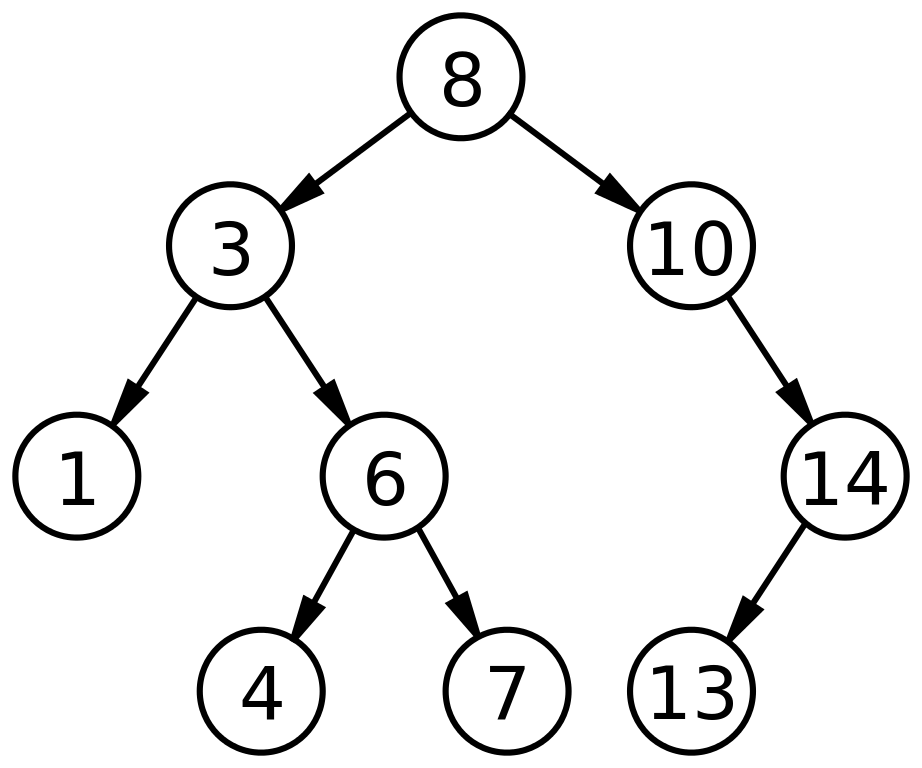
\includegraphics[width=0.5\textwidth]{figures/btree.png}\\
		\hspace*{15pt}\hbox{\scriptsize Image By:\thinspace{\itshape Derrick Coetzee}}
		% https://en.wikipedia.org/wiki/File:Binary_search_tree.svg
	\end{center}
\end{frame}

\begin{frame}
	\frametitle{Binary Search Trees}
	
	\begin{block}{Binary \alert{Search} Trees}
		\begin{itemize}
			\item Every node has at most 2 children.
				\pause
			\item The left descendants have a smaller value than the node.
			\item The right descendants have a larger value than the node.
		\end{itemize}
	\end{block}	
	\pause
	\begin{columns}
		\column{0.455\textwidth}

		\begin{tikzpicture}[
			level distance = 2.5em,
			level 1/.style={sibling distance=9em},
			level 2/.style={sibling distance=4.5em},
			level 3/.style={sibling distance=2.25em},
			]
			\node[ellipse] (t1) {12}
			child { node[ellipse]   {3}
				child { node[ellipse] {2}}
				child { node[ellipse] {9}}
			}
			child { node[ellipse]   {25}
				child { node[ellipse] {14}}
				child { node[ellipse] {29}
					child { node[ellipse] {26}}
					child { node[ellipse] {32}}
				}
			};
		\end{tikzpicture}
		\column{0.455\textwidth}

		\begin{questionblock}{Is it full?}
			Is this tree a binary search tree?
		\end{questionblock}
		\pause
		\begin{answerblock}{}
			Yes :)	
		\end{answerblock}
	\end{columns}
\end{frame}

\begin{frame}
	\frametitle{Searching in a Binary SearchTree}
	
	\vspace{-20pt}
	\begin{overlayarea}{\textwidth}{\textheight}
		\begin{questionblock}{Searching}
			So, how quickly can we search for an item in a Binary Search Tree?
			\only<1>{
			\begin{enumerate}[A.]
				\item $\Theta(\log h)$
				\item $\Theta(h)$
				\item $\Theta(\log n)$
				\item $\Theta(n)$
				\item $\Theta($\textit{I don't know man}$)$
			\end{enumerate}
		}
		\end{questionblock}
		\pause
		\lstinputlisting{code/search_btree.py}
		\pause
	\vspace{-10pt}
		\begin{answerblock}{Only one path}
			So $\Theta(h)$
		\end{answerblock}
	\end{overlayarea}
\end{frame}

\begin{frame}
	\frametitle{MinMaxing}
	
	\begin{overlayarea}{\textwidth}{\textheight}
		\begin{questionblock}{Minmaxing like a real gamer}
			So, how quickly can we find the minimum or maximum in a Binary Search Tree?
			\only<1>{
			\begin{enumerate}[A.]
				\item $\Theta(\log h)$
				\item $\Theta(h)$
				\item $\Theta(\log n)$
				\item $\Theta(n)$
				\item $\Theta($\textit{Something?}$)$
			\end{enumerate}
		}
		\end{questionblock}
		\pause
		\lstinputlisting{code/minmax_btree.py}
		\pause
		\begin{answerblock}{Only one path}
			So $\Theta(h)$
		\end{answerblock}
	\end{overlayarea}
\end{frame}

\begin{frame}
	\frametitle{Inserting or Deleting an item}

	\begin{block}{Inserting an item}
		Find the right place in $\Theta(h)$ time, then put it there.
	\end{block}	

	\pause
	\begin{block}{Deleting an item}
		Find the item in $\Theta(h)$ time, then move either the left or right child up one level (and continue this down the
		path to a leaf).
	\end{block}	
	\pause
		\begin{block}{Sorting the list}
			Oh and by the way, this is where the in-order traversal can get us a sorted list of all items in the tree!
		\end{block}	
\end{frame}


\begin{frame}
	\frametitle{So in summary}
	\begin{tabular}{r | l}
		Operation & Time \\
		\midrule
		Insert & $\Theta(h)$ \\
		Delete & $\Theta(h)$ \\
		Search & $\Theta(h)$ \\
		Min & $\Theta(h)$ \\
		Max & $\Theta(h)$ \\
	\end{tabular}
	\pause	
	\begin{questionblock}{So how bad is it?}
		What is the worst-case $h$, and how do we get that?
	\end{questionblock}
	\pause
	\begin{answerblock}{Inserting a sorted list}
		Insert a sorted list, and what happens? \\
		\pause 
		We get a tree with only right children (or only left if the list is sorted descendingly).
	\end{answerblock}
	
\end{frame}
